
% Default to the notebook output style

    


% Inherit from the specified cell style.




    
\documentclass[11pt]{article}

    
    
    \usepackage[T1]{fontenc}
    % Nicer default font (+ math font) than Computer Modern for most use cases
    \usepackage{mathpazo}

    % Basic figure setup, for now with no caption control since it's done
    % automatically by Pandoc (which extracts ![](path) syntax from Markdown).
    \usepackage{graphicx}
    % We will generate all images so they have a width \maxwidth. This means
    % that they will get their normal width if they fit onto the page, but
    % are scaled down if they would overflow the margins.
    \makeatletter
    \def\maxwidth{\ifdim\Gin@nat@width>\linewidth\linewidth
    \else\Gin@nat@width\fi}
    \makeatother
    \let\Oldincludegraphics\includegraphics
    % Set max figure width to be 80% of text width, for now hardcoded.
    \renewcommand{\includegraphics}[1]{\Oldincludegraphics[width=.8\maxwidth]{#1}}
    % Ensure that by default, figures have no caption (until we provide a
    % proper Figure object with a Caption API and a way to capture that
    % in the conversion process - todo).
    \usepackage{caption}
    \DeclareCaptionLabelFormat{nolabel}{}
    \captionsetup{labelformat=nolabel}

    \usepackage{adjustbox} % Used to constrain images to a maximum size 
    \usepackage{xcolor} % Allow colors to be defined
    \usepackage{enumerate} % Needed for markdown enumerations to work
    \usepackage{geometry} % Used to adjust the document margins
    \usepackage{amsmath} % Equations
    \usepackage{amssymb} % Equations
    \usepackage{textcomp} % defines textquotesingle
    % Hack from http://tex.stackexchange.com/a/47451/13684:
    \AtBeginDocument{%
        \def\PYZsq{\textquotesingle}% Upright quotes in Pygmentized code
    }
    \usepackage{upquote} % Upright quotes for verbatim code
    \usepackage{eurosym} % defines \euro
    \usepackage[mathletters]{ucs} % Extended unicode (utf-8) support
    \usepackage[utf8x]{inputenc} % Allow utf-8 characters in the tex document
    \usepackage{fancyvrb} % verbatim replacement that allows latex
    \usepackage{grffile} % extends the file name processing of package graphics 
                         % to support a larger range 
    % The hyperref package gives us a pdf with properly built
    % internal navigation ('pdf bookmarks' for the table of contents,
    % internal cross-reference links, web links for URLs, etc.)
    \usepackage{hyperref}
    \usepackage{longtable} % longtable support required by pandoc >1.10
    \usepackage{booktabs}  % table support for pandoc > 1.12.2
    \usepackage[inline]{enumitem} % IRkernel/repr support (it uses the enumerate* environment)
    \usepackage[normalem]{ulem} % ulem is needed to support strikethroughs (\sout)
                                % normalem makes italics be italics, not underlines
    

    
    
    % Colors for the hyperref package
    \definecolor{urlcolor}{rgb}{0,.145,.698}
    \definecolor{linkcolor}{rgb}{.71,0.21,0.01}
    \definecolor{citecolor}{rgb}{.12,.54,.11}

    % ANSI colors
    \definecolor{ansi-black}{HTML}{3E424D}
    \definecolor{ansi-black-intense}{HTML}{282C36}
    \definecolor{ansi-red}{HTML}{E75C58}
    \definecolor{ansi-red-intense}{HTML}{B22B31}
    \definecolor{ansi-green}{HTML}{00A250}
    \definecolor{ansi-green-intense}{HTML}{007427}
    \definecolor{ansi-yellow}{HTML}{DDB62B}
    \definecolor{ansi-yellow-intense}{HTML}{B27D12}
    \definecolor{ansi-blue}{HTML}{208FFB}
    \definecolor{ansi-blue-intense}{HTML}{0065CA}
    \definecolor{ansi-magenta}{HTML}{D160C4}
    \definecolor{ansi-magenta-intense}{HTML}{A03196}
    \definecolor{ansi-cyan}{HTML}{60C6C8}
    \definecolor{ansi-cyan-intense}{HTML}{258F8F}
    \definecolor{ansi-white}{HTML}{C5C1B4}
    \definecolor{ansi-white-intense}{HTML}{A1A6B2}

    % commands and environments needed by pandoc snippets
    % extracted from the output of `pandoc -s`
    \providecommand{\tightlist}{%
      \setlength{\itemsep}{0pt}\setlength{\parskip}{0pt}}
    \DefineVerbatimEnvironment{Highlighting}{Verbatim}{commandchars=\\\{\}}
    % Add ',fontsize=\small' for more characters per line
    \newenvironment{Shaded}{}{}
    \newcommand{\KeywordTok}[1]{\textcolor[rgb]{0.00,0.44,0.13}{\textbf{{#1}}}}
    \newcommand{\DataTypeTok}[1]{\textcolor[rgb]{0.56,0.13,0.00}{{#1}}}
    \newcommand{\DecValTok}[1]{\textcolor[rgb]{0.25,0.63,0.44}{{#1}}}
    \newcommand{\BaseNTok}[1]{\textcolor[rgb]{0.25,0.63,0.44}{{#1}}}
    \newcommand{\FloatTok}[1]{\textcolor[rgb]{0.25,0.63,0.44}{{#1}}}
    \newcommand{\CharTok}[1]{\textcolor[rgb]{0.25,0.44,0.63}{{#1}}}
    \newcommand{\StringTok}[1]{\textcolor[rgb]{0.25,0.44,0.63}{{#1}}}
    \newcommand{\CommentTok}[1]{\textcolor[rgb]{0.38,0.63,0.69}{\textit{{#1}}}}
    \newcommand{\OtherTok}[1]{\textcolor[rgb]{0.00,0.44,0.13}{{#1}}}
    \newcommand{\AlertTok}[1]{\textcolor[rgb]{1.00,0.00,0.00}{\textbf{{#1}}}}
    \newcommand{\FunctionTok}[1]{\textcolor[rgb]{0.02,0.16,0.49}{{#1}}}
    \newcommand{\RegionMarkerTok}[1]{{#1}}
    \newcommand{\ErrorTok}[1]{\textcolor[rgb]{1.00,0.00,0.00}{\textbf{{#1}}}}
    \newcommand{\NormalTok}[1]{{#1}}
    
    % Additional commands for more recent versions of Pandoc
    \newcommand{\ConstantTok}[1]{\textcolor[rgb]{0.53,0.00,0.00}{{#1}}}
    \newcommand{\SpecialCharTok}[1]{\textcolor[rgb]{0.25,0.44,0.63}{{#1}}}
    \newcommand{\VerbatimStringTok}[1]{\textcolor[rgb]{0.25,0.44,0.63}{{#1}}}
    \newcommand{\SpecialStringTok}[1]{\textcolor[rgb]{0.73,0.40,0.53}{{#1}}}
    \newcommand{\ImportTok}[1]{{#1}}
    \newcommand{\DocumentationTok}[1]{\textcolor[rgb]{0.73,0.13,0.13}{\textit{{#1}}}}
    \newcommand{\AnnotationTok}[1]{\textcolor[rgb]{0.38,0.63,0.69}{\textbf{\textit{{#1}}}}}
    \newcommand{\CommentVarTok}[1]{\textcolor[rgb]{0.38,0.63,0.69}{\textbf{\textit{{#1}}}}}
    \newcommand{\VariableTok}[1]{\textcolor[rgb]{0.10,0.09,0.49}{{#1}}}
    \newcommand{\ControlFlowTok}[1]{\textcolor[rgb]{0.00,0.44,0.13}{\textbf{{#1}}}}
    \newcommand{\OperatorTok}[1]{\textcolor[rgb]{0.40,0.40,0.40}{{#1}}}
    \newcommand{\BuiltInTok}[1]{{#1}}
    \newcommand{\ExtensionTok}[1]{{#1}}
    \newcommand{\PreprocessorTok}[1]{\textcolor[rgb]{0.74,0.48,0.00}{{#1}}}
    \newcommand{\AttributeTok}[1]{\textcolor[rgb]{0.49,0.56,0.16}{{#1}}}
    \newcommand{\InformationTok}[1]{\textcolor[rgb]{0.38,0.63,0.69}{\textbf{\textit{{#1}}}}}
    \newcommand{\WarningTok}[1]{\textcolor[rgb]{0.38,0.63,0.69}{\textbf{\textit{{#1}}}}}
    
    
    % Define a nice break command that doesn't care if a line doesn't already
    % exist.
    \def\br{\hspace*{\fill} \\* }
    % Math Jax compatability definitions
    \def\gt{>}
    \def\lt{<}
    % Document parameters
    \title{Datadog Hiring Engineers Exercise}
    
    
    

    % Pygments definitions
    
\makeatletter
\def\PY@reset{\let\PY@it=\relax \let\PY@bf=\relax%
    \let\PY@ul=\relax \let\PY@tc=\relax%
    \let\PY@bc=\relax \let\PY@ff=\relax}
\def\PY@tok#1{\csname PY@tok@#1\endcsname}
\def\PY@toks#1+{\ifx\relax#1\empty\else%
    \PY@tok{#1}\expandafter\PY@toks\fi}
\def\PY@do#1{\PY@bc{\PY@tc{\PY@ul{%
    \PY@it{\PY@bf{\PY@ff{#1}}}}}}}
\def\PY#1#2{\PY@reset\PY@toks#1+\relax+\PY@do{#2}}

\expandafter\def\csname PY@tok@w\endcsname{\def\PY@tc##1{\textcolor[rgb]{0.73,0.73,0.73}{##1}}}
\expandafter\def\csname PY@tok@c\endcsname{\let\PY@it=\textit\def\PY@tc##1{\textcolor[rgb]{0.25,0.50,0.50}{##1}}}
\expandafter\def\csname PY@tok@cp\endcsname{\def\PY@tc##1{\textcolor[rgb]{0.74,0.48,0.00}{##1}}}
\expandafter\def\csname PY@tok@k\endcsname{\let\PY@bf=\textbf\def\PY@tc##1{\textcolor[rgb]{0.00,0.50,0.00}{##1}}}
\expandafter\def\csname PY@tok@kp\endcsname{\def\PY@tc##1{\textcolor[rgb]{0.00,0.50,0.00}{##1}}}
\expandafter\def\csname PY@tok@kt\endcsname{\def\PY@tc##1{\textcolor[rgb]{0.69,0.00,0.25}{##1}}}
\expandafter\def\csname PY@tok@o\endcsname{\def\PY@tc##1{\textcolor[rgb]{0.40,0.40,0.40}{##1}}}
\expandafter\def\csname PY@tok@ow\endcsname{\let\PY@bf=\textbf\def\PY@tc##1{\textcolor[rgb]{0.67,0.13,1.00}{##1}}}
\expandafter\def\csname PY@tok@nb\endcsname{\def\PY@tc##1{\textcolor[rgb]{0.00,0.50,0.00}{##1}}}
\expandafter\def\csname PY@tok@nf\endcsname{\def\PY@tc##1{\textcolor[rgb]{0.00,0.00,1.00}{##1}}}
\expandafter\def\csname PY@tok@nc\endcsname{\let\PY@bf=\textbf\def\PY@tc##1{\textcolor[rgb]{0.00,0.00,1.00}{##1}}}
\expandafter\def\csname PY@tok@nn\endcsname{\let\PY@bf=\textbf\def\PY@tc##1{\textcolor[rgb]{0.00,0.00,1.00}{##1}}}
\expandafter\def\csname PY@tok@ne\endcsname{\let\PY@bf=\textbf\def\PY@tc##1{\textcolor[rgb]{0.82,0.25,0.23}{##1}}}
\expandafter\def\csname PY@tok@nv\endcsname{\def\PY@tc##1{\textcolor[rgb]{0.10,0.09,0.49}{##1}}}
\expandafter\def\csname PY@tok@no\endcsname{\def\PY@tc##1{\textcolor[rgb]{0.53,0.00,0.00}{##1}}}
\expandafter\def\csname PY@tok@nl\endcsname{\def\PY@tc##1{\textcolor[rgb]{0.63,0.63,0.00}{##1}}}
\expandafter\def\csname PY@tok@ni\endcsname{\let\PY@bf=\textbf\def\PY@tc##1{\textcolor[rgb]{0.60,0.60,0.60}{##1}}}
\expandafter\def\csname PY@tok@na\endcsname{\def\PY@tc##1{\textcolor[rgb]{0.49,0.56,0.16}{##1}}}
\expandafter\def\csname PY@tok@nt\endcsname{\let\PY@bf=\textbf\def\PY@tc##1{\textcolor[rgb]{0.00,0.50,0.00}{##1}}}
\expandafter\def\csname PY@tok@nd\endcsname{\def\PY@tc##1{\textcolor[rgb]{0.67,0.13,1.00}{##1}}}
\expandafter\def\csname PY@tok@s\endcsname{\def\PY@tc##1{\textcolor[rgb]{0.73,0.13,0.13}{##1}}}
\expandafter\def\csname PY@tok@sd\endcsname{\let\PY@it=\textit\def\PY@tc##1{\textcolor[rgb]{0.73,0.13,0.13}{##1}}}
\expandafter\def\csname PY@tok@si\endcsname{\let\PY@bf=\textbf\def\PY@tc##1{\textcolor[rgb]{0.73,0.40,0.53}{##1}}}
\expandafter\def\csname PY@tok@se\endcsname{\let\PY@bf=\textbf\def\PY@tc##1{\textcolor[rgb]{0.73,0.40,0.13}{##1}}}
\expandafter\def\csname PY@tok@sr\endcsname{\def\PY@tc##1{\textcolor[rgb]{0.73,0.40,0.53}{##1}}}
\expandafter\def\csname PY@tok@ss\endcsname{\def\PY@tc##1{\textcolor[rgb]{0.10,0.09,0.49}{##1}}}
\expandafter\def\csname PY@tok@sx\endcsname{\def\PY@tc##1{\textcolor[rgb]{0.00,0.50,0.00}{##1}}}
\expandafter\def\csname PY@tok@m\endcsname{\def\PY@tc##1{\textcolor[rgb]{0.40,0.40,0.40}{##1}}}
\expandafter\def\csname PY@tok@gh\endcsname{\let\PY@bf=\textbf\def\PY@tc##1{\textcolor[rgb]{0.00,0.00,0.50}{##1}}}
\expandafter\def\csname PY@tok@gu\endcsname{\let\PY@bf=\textbf\def\PY@tc##1{\textcolor[rgb]{0.50,0.00,0.50}{##1}}}
\expandafter\def\csname PY@tok@gd\endcsname{\def\PY@tc##1{\textcolor[rgb]{0.63,0.00,0.00}{##1}}}
\expandafter\def\csname PY@tok@gi\endcsname{\def\PY@tc##1{\textcolor[rgb]{0.00,0.63,0.00}{##1}}}
\expandafter\def\csname PY@tok@gr\endcsname{\def\PY@tc##1{\textcolor[rgb]{1.00,0.00,0.00}{##1}}}
\expandafter\def\csname PY@tok@ge\endcsname{\let\PY@it=\textit}
\expandafter\def\csname PY@tok@gs\endcsname{\let\PY@bf=\textbf}
\expandafter\def\csname PY@tok@gp\endcsname{\let\PY@bf=\textbf\def\PY@tc##1{\textcolor[rgb]{0.00,0.00,0.50}{##1}}}
\expandafter\def\csname PY@tok@go\endcsname{\def\PY@tc##1{\textcolor[rgb]{0.53,0.53,0.53}{##1}}}
\expandafter\def\csname PY@tok@gt\endcsname{\def\PY@tc##1{\textcolor[rgb]{0.00,0.27,0.87}{##1}}}
\expandafter\def\csname PY@tok@err\endcsname{\def\PY@bc##1{\setlength{\fboxsep}{0pt}\fcolorbox[rgb]{1.00,0.00,0.00}{1,1,1}{\strut ##1}}}
\expandafter\def\csname PY@tok@kc\endcsname{\let\PY@bf=\textbf\def\PY@tc##1{\textcolor[rgb]{0.00,0.50,0.00}{##1}}}
\expandafter\def\csname PY@tok@kd\endcsname{\let\PY@bf=\textbf\def\PY@tc##1{\textcolor[rgb]{0.00,0.50,0.00}{##1}}}
\expandafter\def\csname PY@tok@kn\endcsname{\let\PY@bf=\textbf\def\PY@tc##1{\textcolor[rgb]{0.00,0.50,0.00}{##1}}}
\expandafter\def\csname PY@tok@kr\endcsname{\let\PY@bf=\textbf\def\PY@tc##1{\textcolor[rgb]{0.00,0.50,0.00}{##1}}}
\expandafter\def\csname PY@tok@bp\endcsname{\def\PY@tc##1{\textcolor[rgb]{0.00,0.50,0.00}{##1}}}
\expandafter\def\csname PY@tok@fm\endcsname{\def\PY@tc##1{\textcolor[rgb]{0.00,0.00,1.00}{##1}}}
\expandafter\def\csname PY@tok@vc\endcsname{\def\PY@tc##1{\textcolor[rgb]{0.10,0.09,0.49}{##1}}}
\expandafter\def\csname PY@tok@vg\endcsname{\def\PY@tc##1{\textcolor[rgb]{0.10,0.09,0.49}{##1}}}
\expandafter\def\csname PY@tok@vi\endcsname{\def\PY@tc##1{\textcolor[rgb]{0.10,0.09,0.49}{##1}}}
\expandafter\def\csname PY@tok@vm\endcsname{\def\PY@tc##1{\textcolor[rgb]{0.10,0.09,0.49}{##1}}}
\expandafter\def\csname PY@tok@sa\endcsname{\def\PY@tc##1{\textcolor[rgb]{0.73,0.13,0.13}{##1}}}
\expandafter\def\csname PY@tok@sb\endcsname{\def\PY@tc##1{\textcolor[rgb]{0.73,0.13,0.13}{##1}}}
\expandafter\def\csname PY@tok@sc\endcsname{\def\PY@tc##1{\textcolor[rgb]{0.73,0.13,0.13}{##1}}}
\expandafter\def\csname PY@tok@dl\endcsname{\def\PY@tc##1{\textcolor[rgb]{0.73,0.13,0.13}{##1}}}
\expandafter\def\csname PY@tok@s2\endcsname{\def\PY@tc##1{\textcolor[rgb]{0.73,0.13,0.13}{##1}}}
\expandafter\def\csname PY@tok@sh\endcsname{\def\PY@tc##1{\textcolor[rgb]{0.73,0.13,0.13}{##1}}}
\expandafter\def\csname PY@tok@s1\endcsname{\def\PY@tc##1{\textcolor[rgb]{0.73,0.13,0.13}{##1}}}
\expandafter\def\csname PY@tok@mb\endcsname{\def\PY@tc##1{\textcolor[rgb]{0.40,0.40,0.40}{##1}}}
\expandafter\def\csname PY@tok@mf\endcsname{\def\PY@tc##1{\textcolor[rgb]{0.40,0.40,0.40}{##1}}}
\expandafter\def\csname PY@tok@mh\endcsname{\def\PY@tc##1{\textcolor[rgb]{0.40,0.40,0.40}{##1}}}
\expandafter\def\csname PY@tok@mi\endcsname{\def\PY@tc##1{\textcolor[rgb]{0.40,0.40,0.40}{##1}}}
\expandafter\def\csname PY@tok@il\endcsname{\def\PY@tc##1{\textcolor[rgb]{0.40,0.40,0.40}{##1}}}
\expandafter\def\csname PY@tok@mo\endcsname{\def\PY@tc##1{\textcolor[rgb]{0.40,0.40,0.40}{##1}}}
\expandafter\def\csname PY@tok@ch\endcsname{\let\PY@it=\textit\def\PY@tc##1{\textcolor[rgb]{0.25,0.50,0.50}{##1}}}
\expandafter\def\csname PY@tok@cm\endcsname{\let\PY@it=\textit\def\PY@tc##1{\textcolor[rgb]{0.25,0.50,0.50}{##1}}}
\expandafter\def\csname PY@tok@cpf\endcsname{\let\PY@it=\textit\def\PY@tc##1{\textcolor[rgb]{0.25,0.50,0.50}{##1}}}
\expandafter\def\csname PY@tok@c1\endcsname{\let\PY@it=\textit\def\PY@tc##1{\textcolor[rgb]{0.25,0.50,0.50}{##1}}}
\expandafter\def\csname PY@tok@cs\endcsname{\let\PY@it=\textit\def\PY@tc##1{\textcolor[rgb]{0.25,0.50,0.50}{##1}}}

\def\PYZbs{\char`\\}
\def\PYZus{\char`\_}
\def\PYZob{\char`\{}
\def\PYZcb{\char`\}}
\def\PYZca{\char`\^}
\def\PYZam{\char`\&}
\def\PYZlt{\char`\<}
\def\PYZgt{\char`\>}
\def\PYZsh{\char`\#}
\def\PYZpc{\char`\%}
\def\PYZdl{\char`\$}
\def\PYZhy{\char`\-}
\def\PYZsq{\char`\'}
\def\PYZdq{\char`\"}
\def\PYZti{\char`\~}
% for compatibility with earlier versions
\def\PYZat{@}
\def\PYZlb{[}
\def\PYZrb{]}
\makeatother


    % Exact colors from NB
    \definecolor{incolor}{rgb}{0.0, 0.0, 0.5}
    \definecolor{outcolor}{rgb}{0.545, 0.0, 0.0}



    
    % Prevent overflowing lines due to hard-to-break entities
    \sloppy 
    % Setup hyperref package
    \hypersetup{
      breaklinks=true,  % so long urls are correctly broken across lines
      colorlinks=true,
      urlcolor=urlcolor,
      linkcolor=linkcolor,
      citecolor=citecolor,
      }
    % Slightly bigger margins than the latex defaults
    
    \geometry{verbose,tmargin=1in,bmargin=1in,lmargin=1in,rmargin=1in}
    
    

    \begin{document}
    
    
    \maketitle
    
    

    
    \section{Environment}\label{environment}

    \includegraphics{https://www.vectorlogo.zone/logos/docker/docker-card.png}
This testing was done on a Paperspace VM running Ubuntu 18.04. I had
started with Docker on Windows which appeared adequate at first, and
then caused me trouble. I learned that composed Docker stacks on a local
swarm running on Windows doesn't network the same as Linux environments.

\includegraphics{https://www.windowslatest.com/wp-content/uploads/2017/07/Ubuntu-on-Windows-10-696x348.jpg}
I then tried the "Ubuntu" available in the Windows Store. Everything
worked until I discovered there is no /proc filesystem since it's not
even running the Linux kernel. Not having a /proc filesystem leads to a
strange lack of information when using typical Linux tools. Too much
wasted time on that system!

\includegraphics{https://odsc.com/wp-content/uploads/2018/01/paperspace-logo-300x168.jpeg}
Frustrated, I installed both Ubuntu locally in a Hyper-V VM and spun up
a Paperspace instace. Paperspace encountered errors during provisioning,
so I worked on the slow local install for a while. Once Paperspace
errors resolved, their VM was significantly faster than my local machine
so I stuck that.

    \section{Test Application}\label{test-application}

    I developed a simple api with 6 resources: 3 evil, 3 nice. Since my app
is based on Flask, I used the third-party trace-middleware as desribed
in the
\href{https://docs.datadoghq.com/tracing/setup/python/\#example-simple-tracing}{docs}

\subsubsection{source code in ./api/}\label{source-code-in-.api}

I developed methods to post comments and events.

\begin{figure}
\centering
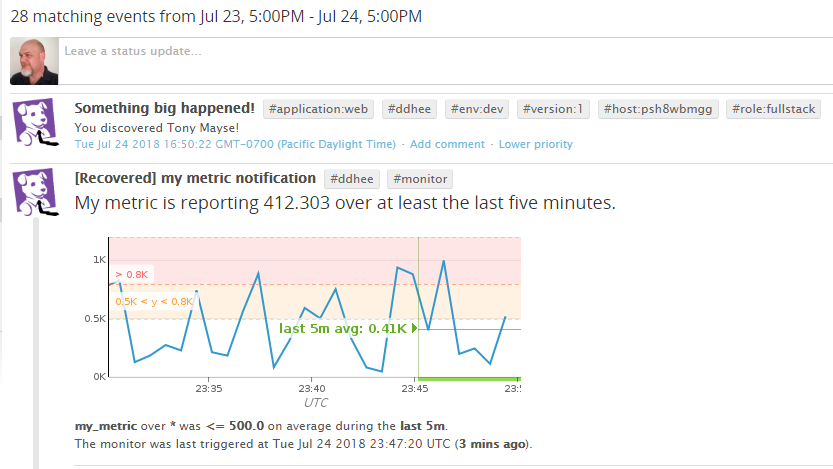
\includegraphics{images/event.png}
\caption{event posted}
\end{figure}

    I installed the datadog agent using the preferred Ubuntu install script.
I noticed that the provided script is prepopulated with necessary keys
and that made installation a breeze.

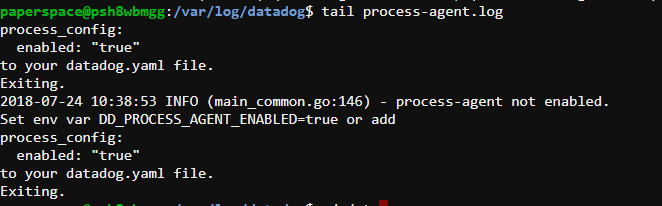
\includegraphics{images/agent_exit.PNG} Something needs fixing, the
agent won't stay running. Looks like I need to enable the agent.

I adjusted the datadog.yaml file to enable the agent and APM and added
tags while I was there. 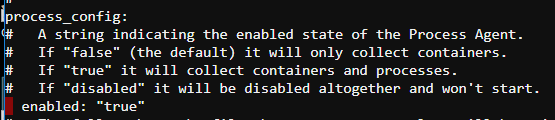
\includegraphics{images/epa.PNG}

\begin{figure}
\centering
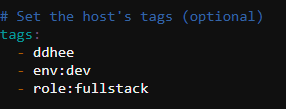
\includegraphics{images/tic.PNG}
\caption{agent exiting}
\end{figure}

Then I verified that the agent was listening on the expected port:

\includegraphics{images/confirm_8126.PNG}

\emph{note: 404 is the expected response.}

And data is coming in!

\begin{figure}
\centering
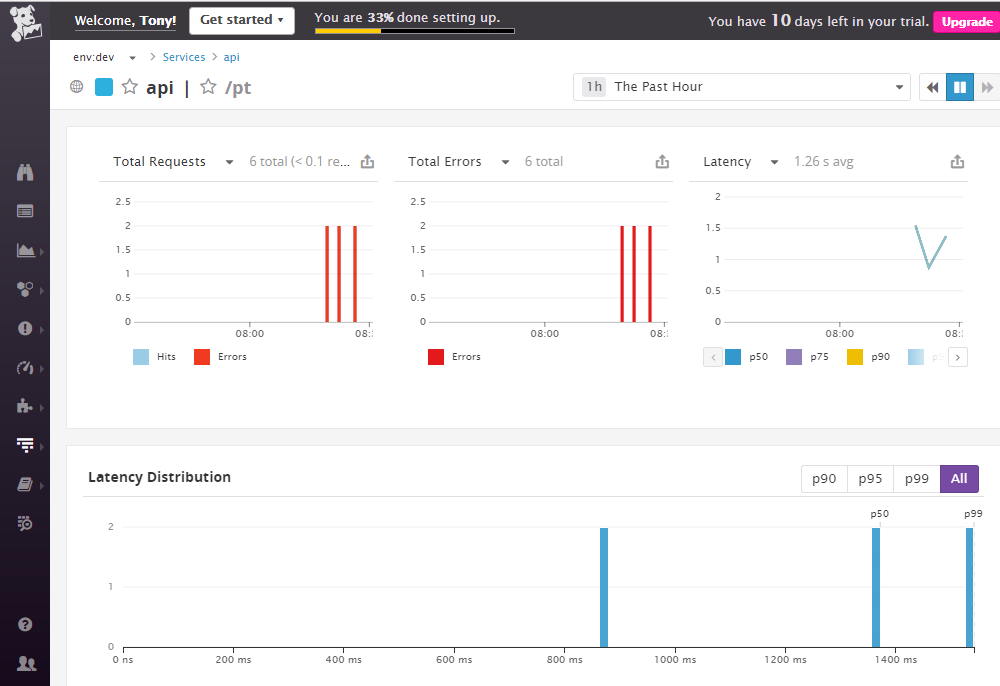
\includegraphics{images/errors.png}
\caption{new data}
\end{figure}

    \section{Custom Check and Metric}\label{custom-check-and-metric}

    I placed the following code in \textbf{/etc/datadog-agent/checks.d/} as

\textbf{my\_metric.py}

    \begin{Verbatim}[commandchars=\\\{\}]
{\color{incolor}In [{\color{incolor} }]:} \PY{k+kn}{from} \PY{n+nn}{checks} \PY{k}{import} \PY{n}{AgentCheck}
        \PY{k+kn}{import} \PY{n+nn}{random}
        \PY{k}{class} \PY{n+nc}{my\PYZus{}metric}\PY{p}{(}\PY{n}{AgentCheck}\PY{p}{)}\PY{p}{:}
            \PY{k}{def} \PY{n+nf}{check}\PY{p}{(}\PY{n+nb+bp}{self}\PY{p}{,} \PY{n}{instance}\PY{p}{)}\PY{p}{:}
                \PY{n}{val} \PY{o}{=} \PY{n}{random}\PY{o}{.}\PY{n}{uniform}\PY{p}{(}\PY{l+m+mi}{0}\PY{p}{,}\PY{l+m+mi}{1000}\PY{p}{)}
                \PY{n+nb+bp}{self}\PY{o}{.}\PY{n}{gauge}\PY{p}{(}\PY{l+s+s1}{\PYZsq{}}\PY{l+s+s1}{my\PYZus{}metric }\PY{l+s+s1}{\PYZsq{}}\PY{p}{,} \PY{n}{val}\PY{p}{,} \PY{n}{tags}\PY{o}{=}\PY{p}{[}\PY{l+s+sa}{u}\PY{l+s+s1}{\PYZsq{}}\PY{l+s+s1}{ddhee}\PY{l+s+s1}{\PYZsq{}}\PY{p}{,}\PY{l+s+sa}{u}\PY{l+s+s1}{\PYZsq{}}\PY{l+s+s1}{maint:tmayse}\PY{l+s+s1}{\PYZsq{}}\PY{p}{]}\PY{p}{)}
\end{Verbatim}


    I placed the following configuration in
\textbf{/etc/datadog-agent/conf.d/my\_metric/} as my\_metric.yaml and
while I was there, I skipped ahead and just configured the check to run
\textbf{not more often than} every 45 seconds.

\textbf{my\_metric.yaml:}

    \begin{Verbatim}[commandchars=\\\{\}]
{\color{incolor}In [{\color{incolor} }]:} \PY{n}{init\PYZus{}config}\PY{p}{:}
        
        \PY{n}{instances}\PY{p}{:}
            \PY{o}{\PYZhy{}} \PY{n}{host}\PY{p}{:} \PY{l+s+s2}{\PYZdq{}}\PY{l+s+s2}{psh8wbmgg}\PY{l+s+s2}{\PYZdq{}}
              \PY{n}{min\PYZus{}collection\PYZus{}interval}\PY{p}{:} \PY{l+m+mi}{45}
\end{Verbatim}


    Checking the config \textbf{sudo service datadog-agent status}

    \begin{figure}
\centering
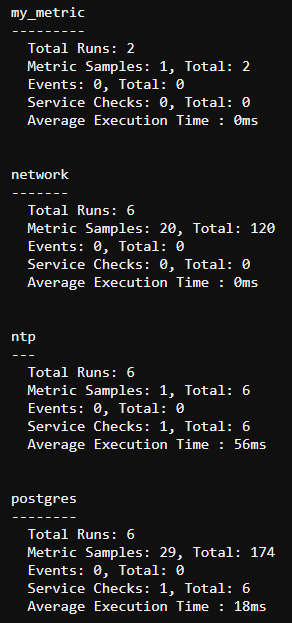
\includegraphics{images/checks.PNG}
\caption{agent config}
\end{figure}

\emph{pleased to find my\_check listed at the top}

Timing confirmed in agent logs: 
\includegraphics{images/45.PNG}

And then, as configured, the check ran:
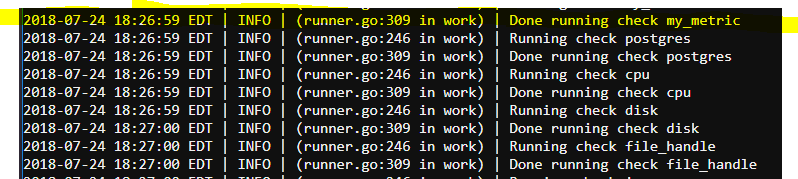
\includegraphics{images/check_ran.PNG}

    \section{Tags on infrastructure}\label{tags-on-infrastructure}

    As show earlier, configured tags: 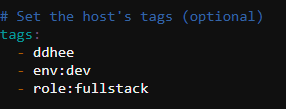
\includegraphics{images/tic.PNG}

\begin{figure}
\centering
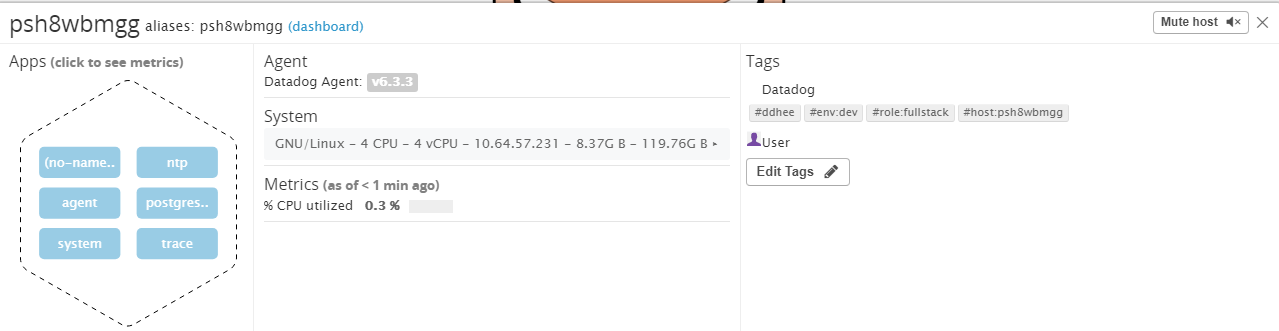
\includegraphics{images/host_tags.PNG}
\caption{host tags in UI}
\end{figure}

Bonus Question Can you change the collection interval without modifying
the Python check file you created? \textbf{see config \& logs above}

\emph{in addition to the tags I configured, an automatic tag was added
identifying the host}

    \section{Database Integration}\label{database-integration}

    I installed Postgresql as it's generally trouble-free. One of my
endpoints (/tfs) stimulates the DB.

The agent is configured by adding postgres.yaml to
/etc/datadog-agent/conf.d/postgres.d/postgres.yaml

\textbf{postgres.yaml:}

    \begin{Verbatim}[commandchars=\\\{\}]
{\color{incolor}In [{\color{incolor} }]:} \PY{o}{\PYZhy{}}\PY{o}{\PYZhy{}}\PY{o}{\PYZhy{}}
        \PY{n}{init\PYZus{}config}\PY{p}{:}
        
        \PY{n}{instances}\PY{p}{:}
          \PY{o}{\PYZhy{}} \PY{n}{host}\PY{p}{:} \PY{n}{localhost}
            \PY{n}{password}\PY{p}{:} \PY{n}{CG4W1mPaET70QWl2TrjYeAlN}
            \PY{n}{port}\PY{p}{:} \PY{l+m+mi}{5432}
            \PY{n}{tags}\PY{p}{:}
              \PY{o}{\PYZhy{}} \PY{n}{ddhee}
              \PY{o}{\PYZhy{}} \PY{l+s+s2}{\PYZdq{}}\PY{l+s+s2}{role:db}\PY{l+s+s2}{\PYZdq{}}
              \PY{o}{\PYZhy{}} \PY{l+s+s2}{\PYZdq{}}\PY{l+s+s2}{description:DDHEE db}\PY{l+s+s2}{\PYZdq{}}
            \PY{n}{username}\PY{p}{:} \PY{n}{datadog}
\end{Verbatim}


    \begin{figure}
\centering
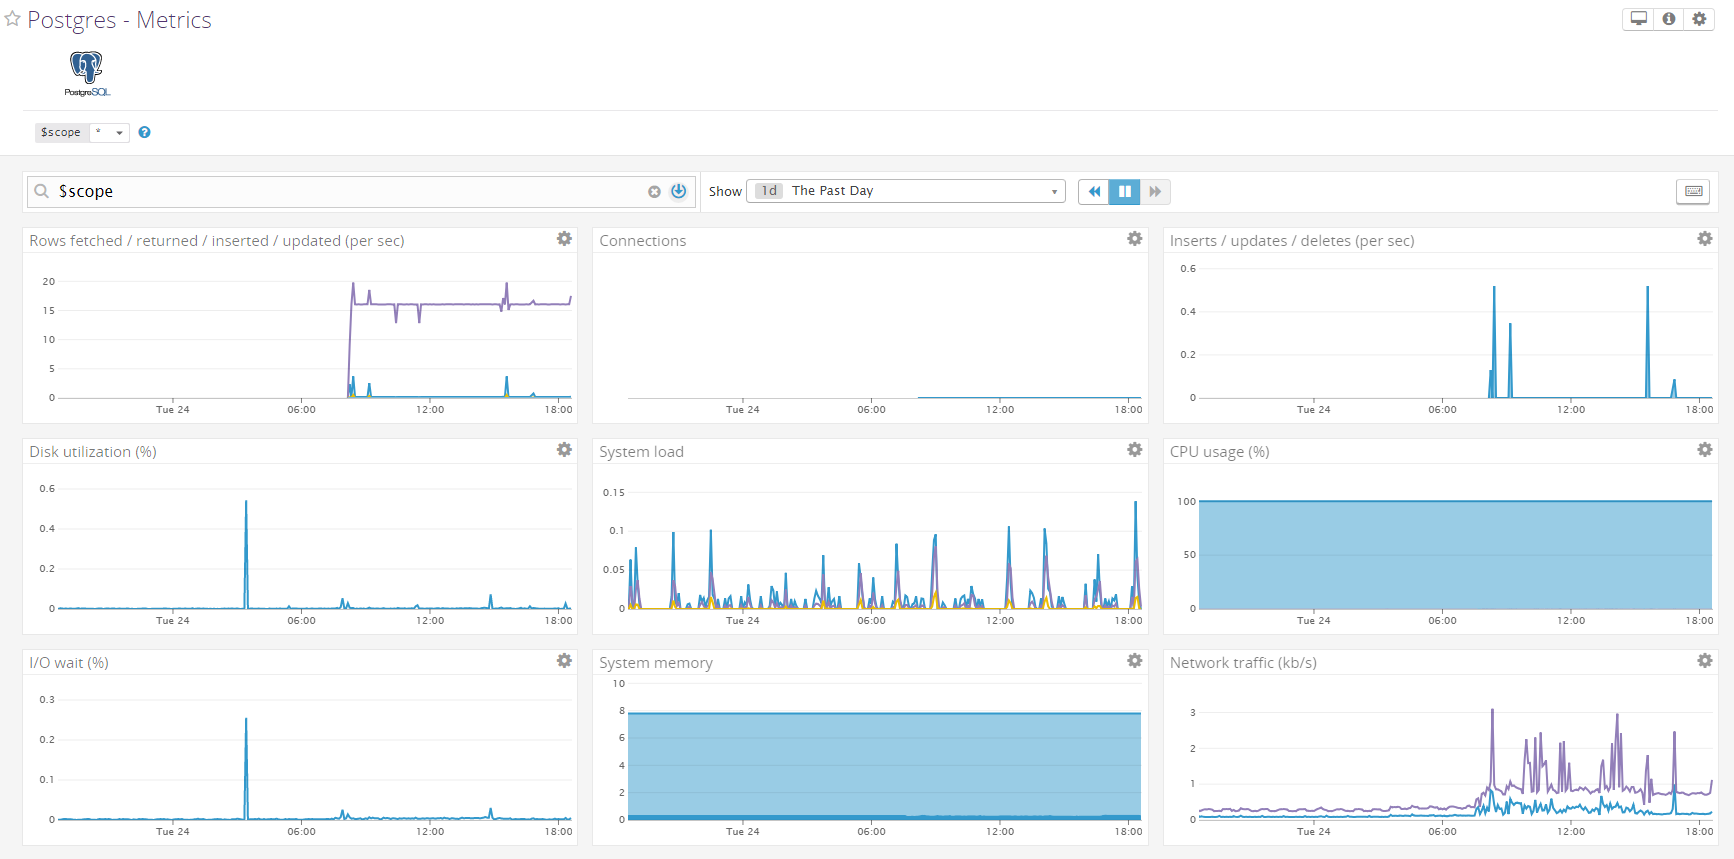
\includegraphics{images/db_dashboard.PNG}
\caption{Database Dashboard}
\end{figure}

\href{https://app.datadoghq.com/screen/integration/235/postgres---overview?page=0\&is_auto=false\&from_ts=1532551260000\&to_ts=1532554860000\&live=true}{Link
to board}

    \section{Timeboard created by API}\label{timeboard-created-by-api}

    I needed 4 tries to get this right. I copied the graph definitions from
the UI dasboard's JSON output. I found that the anomolies method
requires more arguments in a Timeboard. Once I fixed that, my script
worked as-expected.

\textbf{Tmeboard Script:}

    \begin{Verbatim}[commandchars=\\\{\}]
{\color{incolor}In [{\color{incolor} }]:} \PY{c+ch}{\PYZsh{}!/bin/bash}
        
        \PY{n}{curl}  \PY{o}{\PYZhy{}}\PY{n}{X} \PY{n}{POST} \PY{o}{\PYZhy{}}\PY{n}{H} \PY{l+s+s2}{\PYZdq{}}\PY{l+s+s2}{Content\PYZhy{}type: application/json}\PY{l+s+s2}{\PYZdq{}} \PYZbs{}
        \PY{o}{\PYZhy{}}\PY{n}{d} \PY{n+nd}{@graphs}\PY{o}{.}\PY{n}{ddhee}\PY{o}{.}\PY{n}{json} \PY{l+s+s2}{\PYZdq{}}\PY{l+s+s2}{https://api.datadoghq.com/api/v1/dash?api\PYZus{}key=e1dbdaceaf7516f90ef9e2ad5546072e\PYZam{}application\PYZus{}key=25b8d433ca6e9ca99c1ee791e8ece8c67e6a0ec3}\PY{l+s+s2}{\PYZdq{}}
\end{Verbatim}


    \begin{figure}
\centering
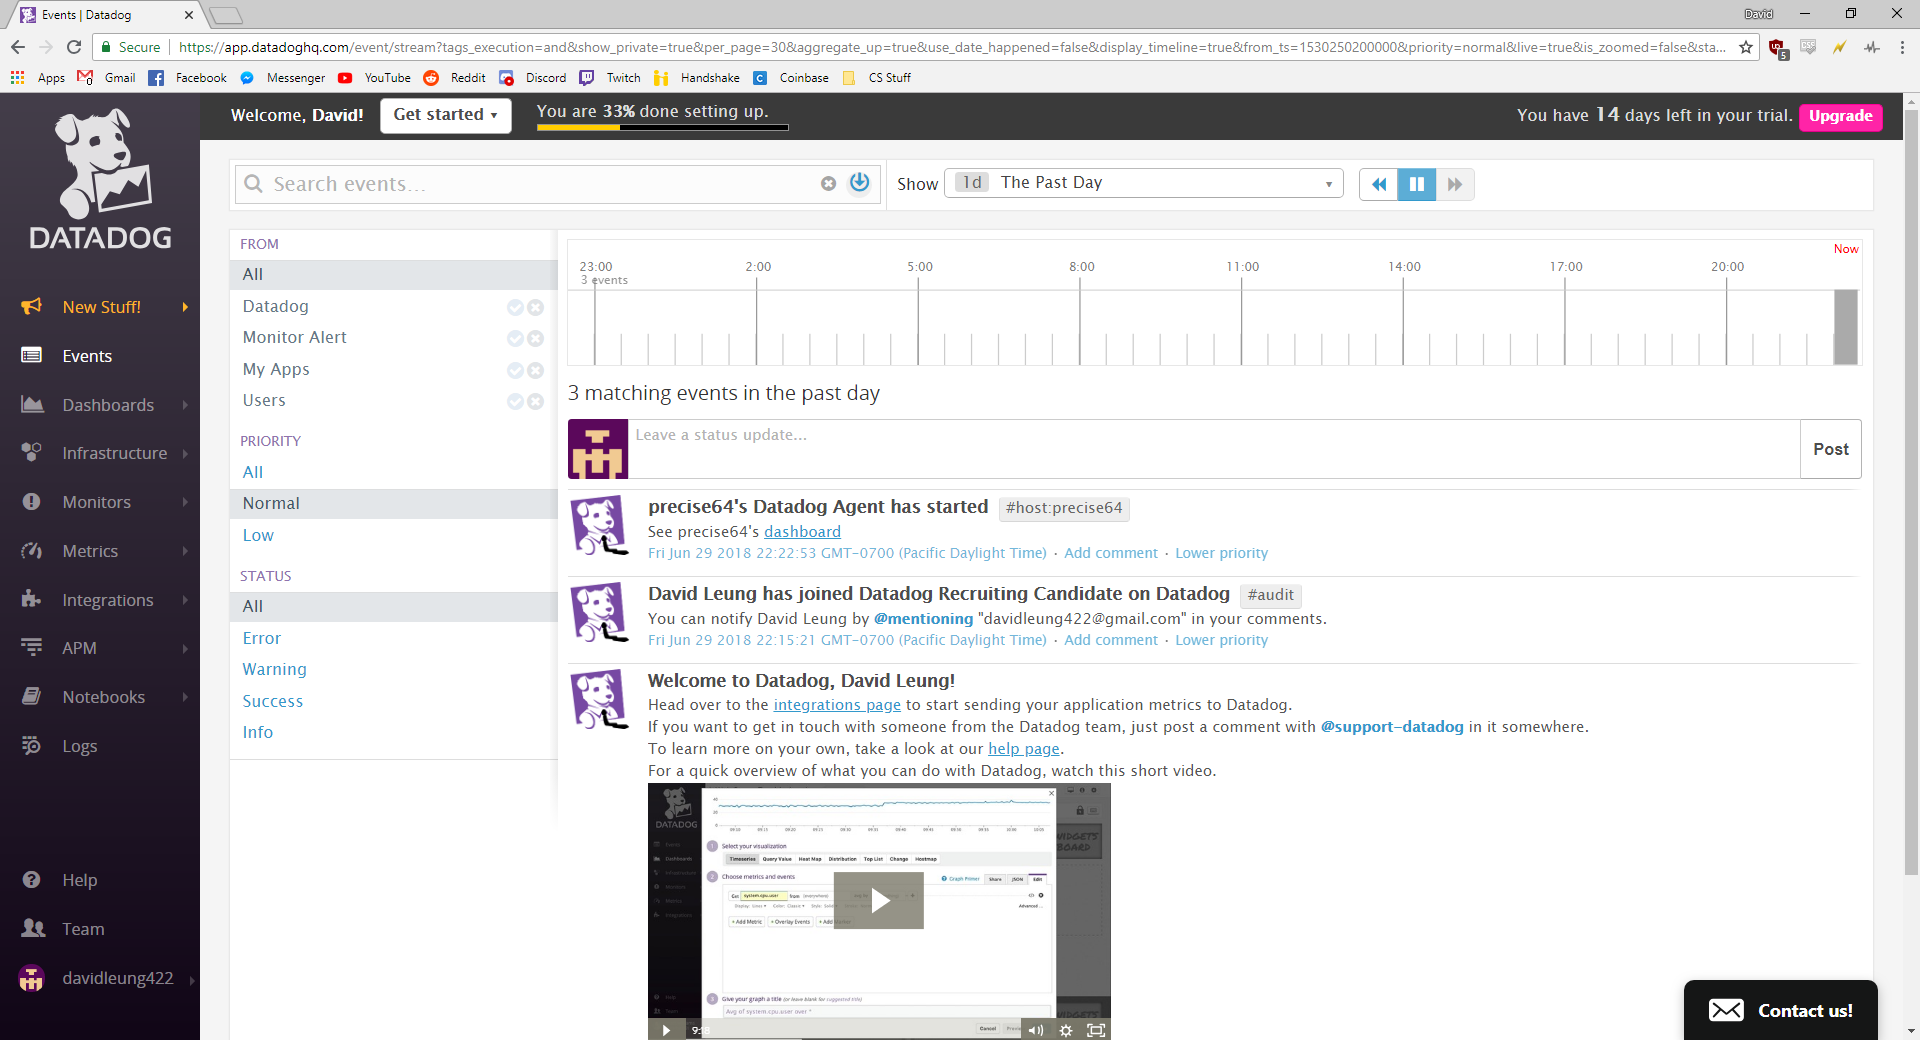
\includegraphics{images/Dashboard.png}
\caption{Dashboard created by API}
\end{figure}

\href{https://app.datadoghq.com/dash/871365/}{dashboard link}

    \section{Timeboard with five minute
window}\label{timeboard-with-five-minute-window}

    This took me a while to figure out. It wasn't immediately obvious to me
that a Screenboard fit the bill. When I came upon
\textbf{\href{https://docs.datadoghq.com/graphing/faq/how-to-transform-a-timeboard-to-a-screenboard-or-vice-versa/}{How
to Transform a Timeboard to a Screenboard or vice versa ?}} which links
to
\href{https://github.com/DataDog/Miscellany/blob/master/dashconverter.py}{this
script} Once my timeboard was converted to a Screenboard, I was able to
set the time to each chart to five minutes.

\textbf{here's the command line util I ran}

    \begin{Verbatim}[commandchars=\\\{\}]
{\color{incolor}In [{\color{incolor} }]:} \PY{n}{python} \PY{n}{dash} \PY{o}{\PYZhy{}}\PY{o}{\PYZhy{}}\PY{n}{api}\PY{o}{\PYZhy{}}\PY{n}{key} \PY{n}{e1dbdaceaf7516f90ef9e2ad5546072e} \PY{o}{\PYZhy{}}\PY{o}{\PYZhy{}}\PY{n}{app}\PY{o}{\PYZhy{}}\PY{n}{key} \PY{l+m+mi}{25}\PY{n}{b8d433ca6e9ca99c1ee791e8ece8c67e6a0ec3} \PY{o}{\PYZhy{}}\PY{o}{\PYZhy{}}\PY{n}{titl}
        \PY{n}{e} \PY{l+s+s2}{\PYZdq{}}\PY{l+s+s2}{From Timeboard}\PY{l+s+s2}{\PYZdq{}} \PY{l+m+mi}{871365}
\end{Verbatim}


    \begin{figure}
\centering
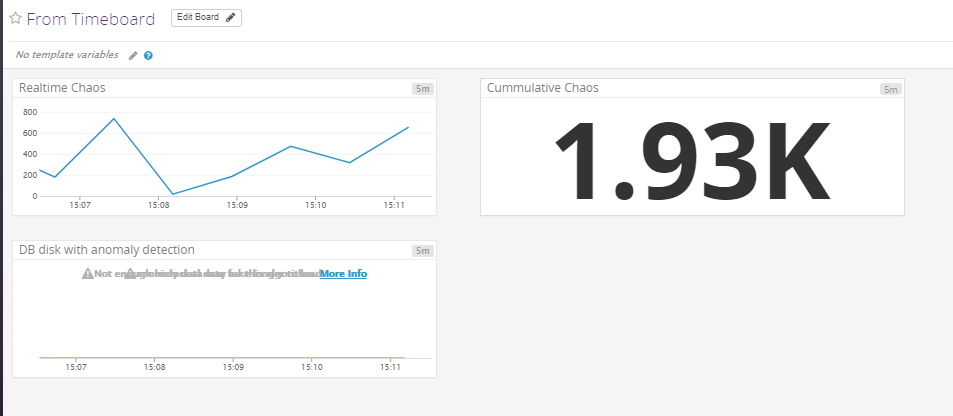
\includegraphics{images/screenboard.png}
\caption{Screenboard Converted by scipt}
\end{figure}

\href{http://app.datadoghq.com/screen/393468}{screenboard link}

\textbf{Bonus Question: What is the Anomaly graph displaying?}

It reads "Not enough historical data for this algorithm."

\emph{note: I didn't explore other algorithms' data requirements.}

I didn't figure out how to send a screenshot, so I sent myself a URL:

\includegraphics{images/atmention.png}

The email I got as a result looked like this:

\includegraphics{images/atmentionemail.png}

    \section{Monitoring Data}\label{monitoring-data}

    This image has all the info necessary to verify notifications: Here's
what I did:

\begin{figure}
\centering
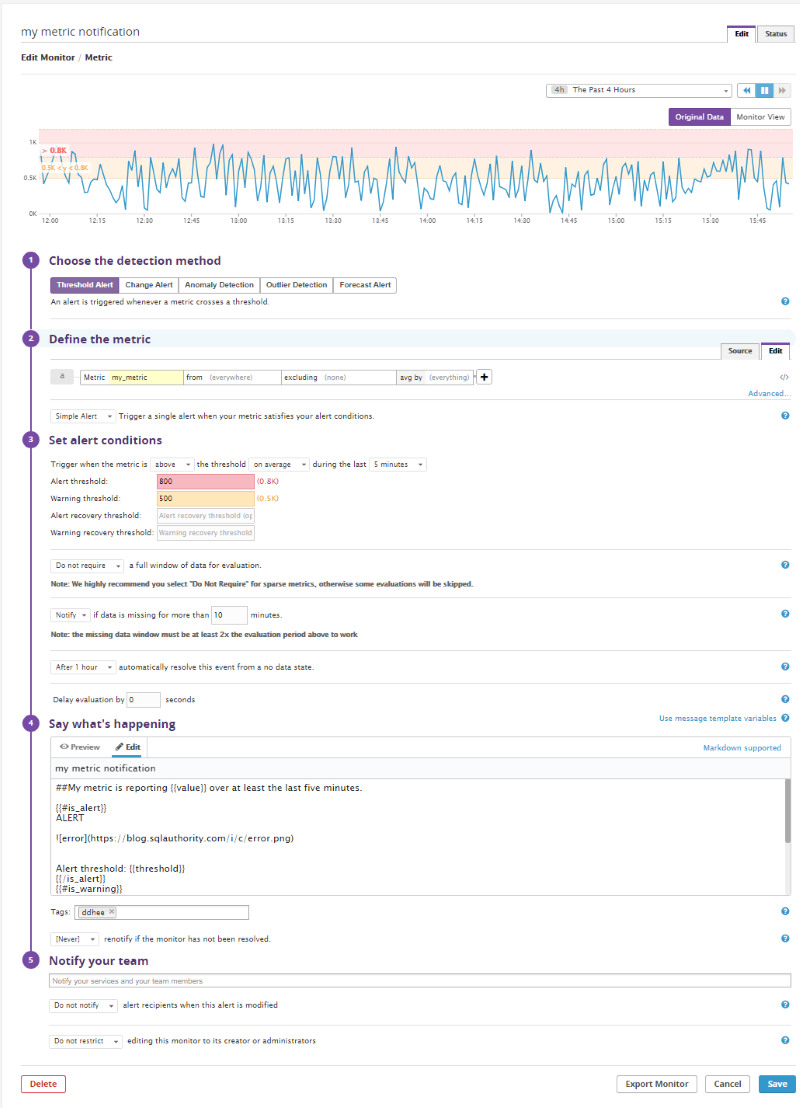
\includegraphics{images/monitorpage.png}
\caption{monitor setup}
\end{figure}

This is very noisy, of course. I'm glad configuring downtimes was part
of the exercise. 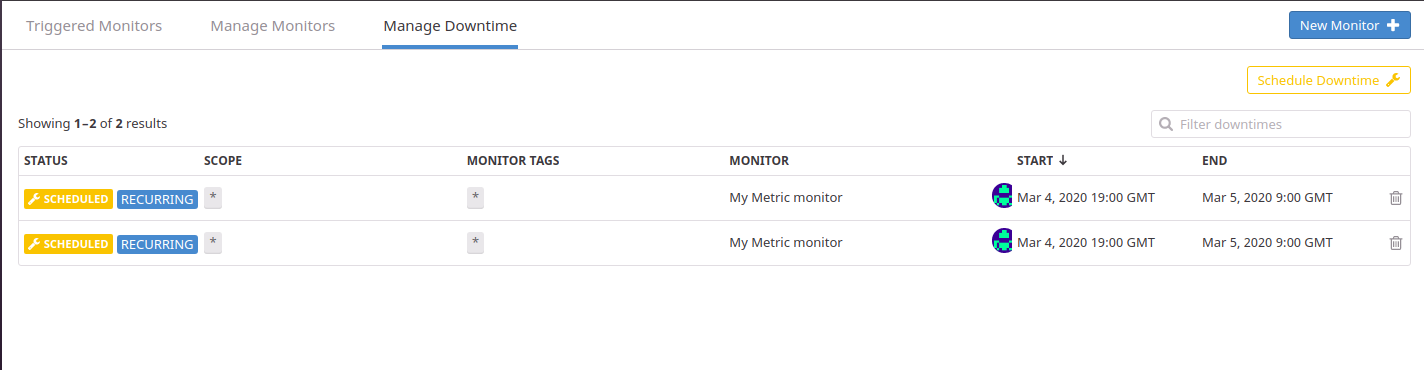
\includegraphics{images/downtime.png}

https://app.datadoghq.com/monitors/5645900

\textbf{note: For the weekend downtime, I was frustrated by an error
that was telling me my start time was too early any time around
midnight. I tried from 11:59PM Fri for two days, but that's clearly not
right as it didn't have the desired effect. It only just now ocurred to
me that the times are UTC. The email was clear about that, but I didn't
read it. A better error message might say "that time is in the past",
but ulitmately, this was my bad.}

\begin{figure}
\centering

\includegraphics{images/schedtime.png}
\caption{downtime}
\end{figure}

In addition to an email, I captured this event in the event stream:

\begin{figure}
\centering
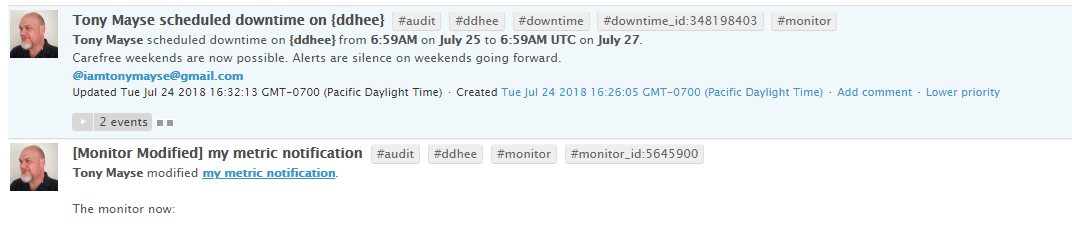
\includegraphics{images/notif.png}
\caption{event in stream}
\end{figure}

I also enable suggested monitors for my API and was alerted
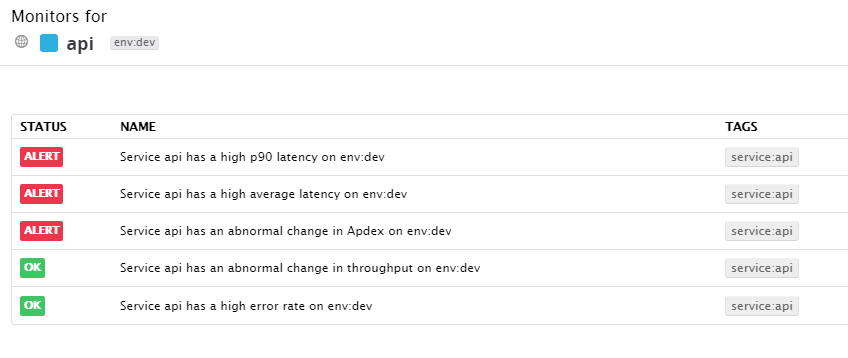
\includegraphics{images/hammer.png}

    \section{Integrated Dashboard}\label{integrated-dashboard}

    https://app.datadoghq.com/dash/871420

Included in this dashboard are process metrics, my\_metric chaos, NTP
offset, and average Apdex by resource.

\begin{figure}
\centering
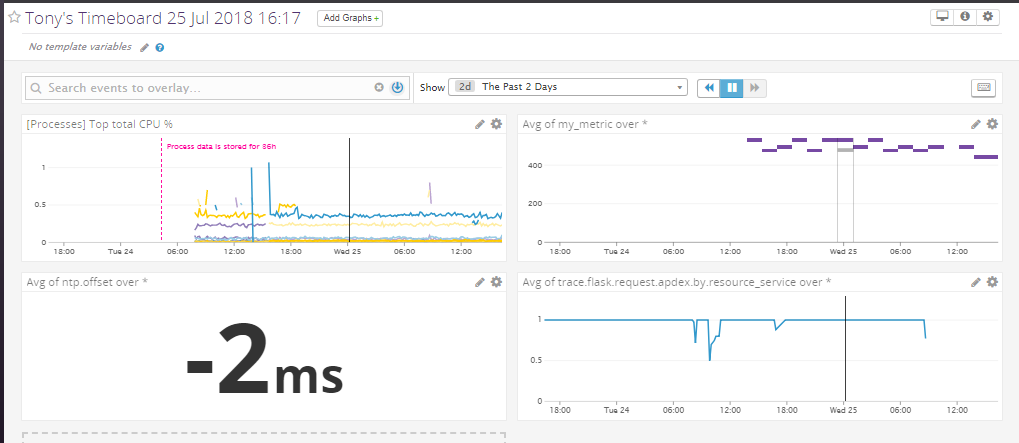
\includegraphics{images/hostandapp.PNG}
\caption{App \& Host metrics}
\end{figure}

\textbf{Bonus Question: What is the difference between a Service and a
Resource?} A service is a group of resources. Short answer: service is
essentially the application and resource is essentially it's
endpoints/methods.

Here's my application's resource list:

\begin{figure}
\centering
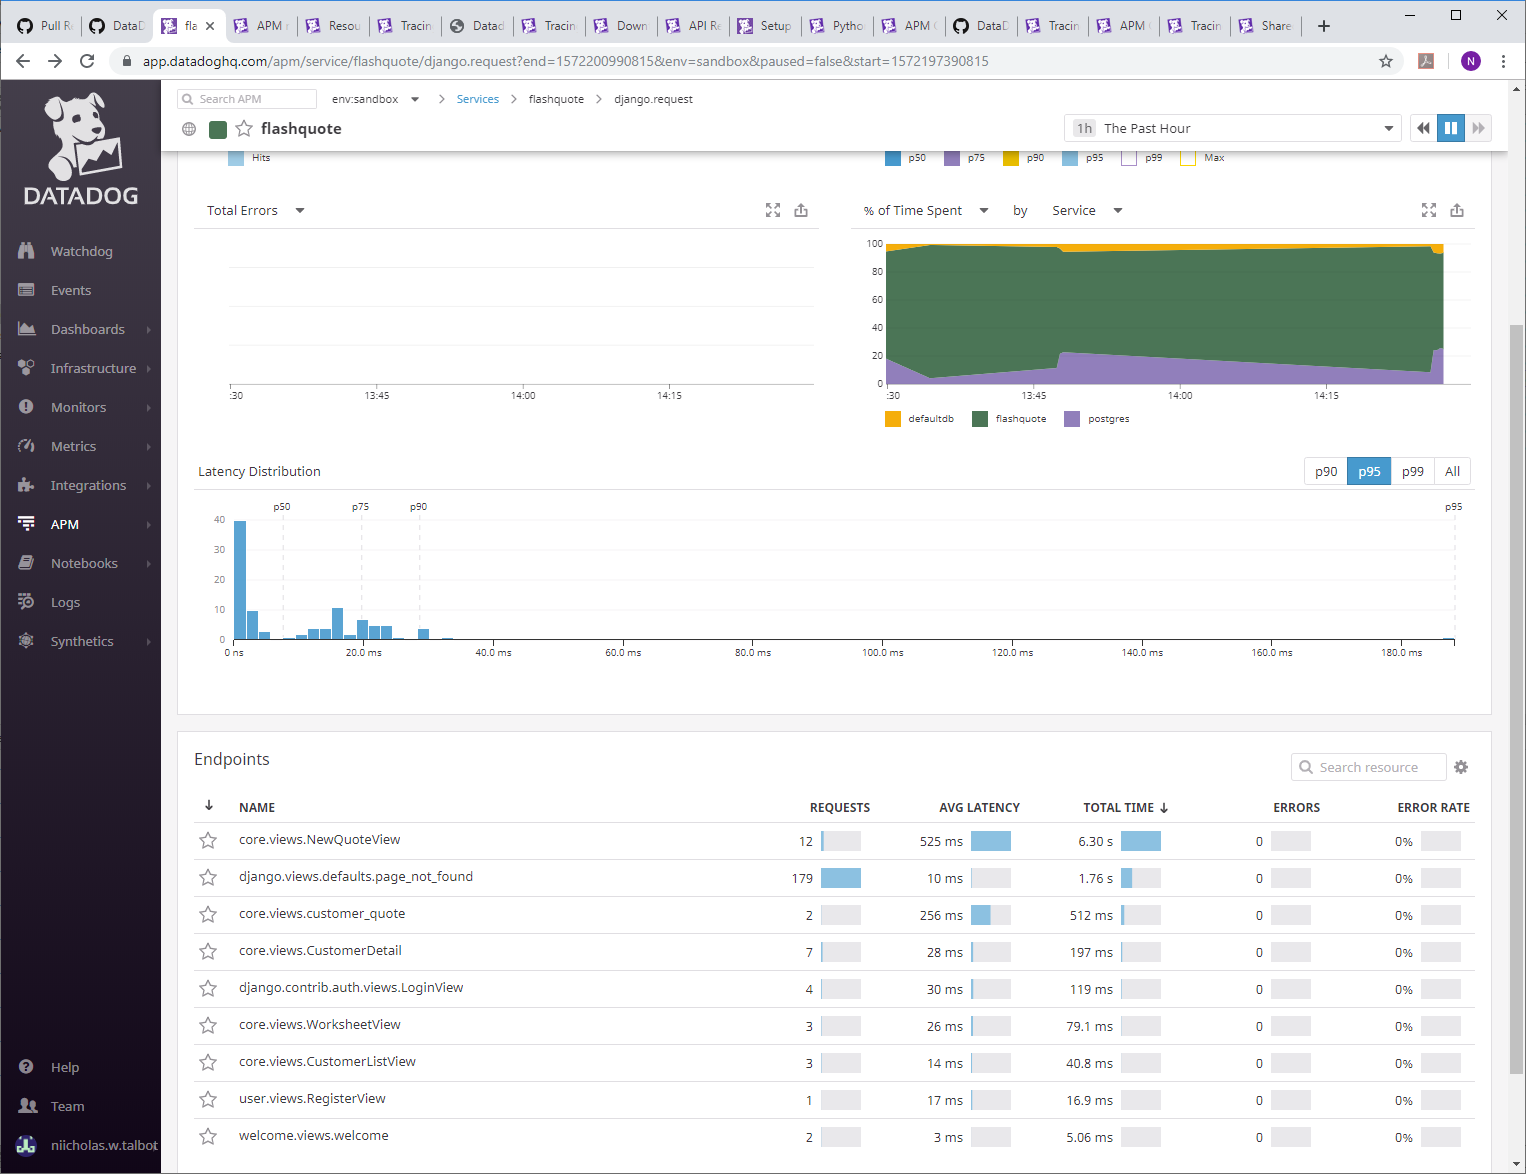
\includegraphics{images/resources.png}
\caption{resource list}
\end{figure}

and here's the service to which they all belong:

\begin{figure}
\centering
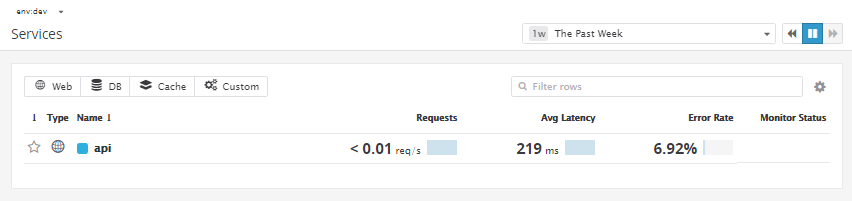
\includegraphics{images/services.png}
\caption{services}
\end{figure}

    \section{Last Question}\label{last-question}

    During my call with Fahim, I already volunteered call center/suport desk
metrics: call volume, hold time, etc. Anomoly detection would be helpful
in addition to developing a more robust view of the enterprise.

Here's a crazy idea that might just work: All on-call engineers track
their location via smartphone or whatever is available. Datadog could
alert the manager if too few engineers are within rapid-response range
of the office.


    % Add a bibliography block to the postdoc
    
    
    
    \end{document}
